\documentclass{beamer}

\usepackage{graphicx}
\usepackage{listings}
\usepackage[utf8]{inputenc}
\usepackage{tikz}
\usetikzlibrary{calc}
\usetikzlibrary{intersections}

%30 min

\lstset{
  basicstyle=\footnotesize,        % the size of the fonts that are used for the code
  breakatwhitespace=true,         % sets if automatic breaks should only happen at whitespace
  breaklines=true,                 % sets automatic line breaking
  commentstyle=\color{green},      % comment style
  keywordstyle=\color{blue},       % keyword style
  language=C++,                    % the language of the code
  numbers=none,                    % where to put the line-numbers; possible values are (none, left, right)
}


\newcommand{\sectiontitle}[1]{
    \section{#1}
    \begin{frame}
        \centering
        \LARGE{#1}
    \end{frame}
}
\newcommand{\subsectiontitle}[1]{
    \subsection{#1}
    \begin{frame}
        \LARGE{#1}
    \end{frame}
}

\newcommand{\inlinecpp}[1]{
    \lstinline[language=C++]{#1}
}


\title[ugtest]{ugtest}
\author{Tobias Trautmann}
\institute{GCSC}

\begin{document}

    \begin{frame}
        \titlepage
    \end{frame}

    \begin{frame}{Outline}
        \tableofcontents
    \end{frame}


    \sectiontitle{Introduction to testing}
        %talk about differneces between debugging and testing
        %talk about coverage and ease of defect localistion
        %systematisch!
        %nicht so viel theorie!!!
        \subsection{Goals}
        \begin{frame}{Goals of testing}
            %nur geteste software erzeugt wert
            %it := Software
            %functional  non-functional
            % testing destructive
           \begin{itemize}
                \item increase trust in its results\pause
                \item make code maintainable\pause
                \item make code refactorable\pause
                \item make it sufficiently robust\pause
                \item check if it performs its functions within an acceptable time\pause
                \item check wether in runs its intended environments
           \end{itemize}
           \Large{$\Rightarrow$ Testing software is a \textbf{necessity}}
        \end{frame}

        \subsection{Defects}
        \begin{frame}{Defects}
            %make an explanation why definition of failure is importat
            %makes it much easier to understand bugs during debugging and
            %allows to set priorities when developing test cases
            % magic numbers
            %fehlerfortpflanzung
            Where do defects come from?\\
            \begin{itemize}
                \item script error (lua)
                \item bug in code
                \item integration
                \item error in design
            \end{itemize}
            Are you responsible for it?\\
            mitigation
            runtime error logging
            
            $\Rightarrow$ Makes clear what to test with which priority

        \end{frame}
        
        \subsection{Efficency}
        \begin{frame}[plain]{Efficency}
            %Talk about each test level, what it does what its for and when to do them
            %effort goes up with pyramid
            %time to develop goes up
            % pesticide paradox\\%bugs become more subtle the more you cover
            % testen für qualität nicht für statistik!!
            % amount of work put into testing 25\%-50\% of total  time!!!!!
            % entwicklungsbegleitendes testen
            \centering
            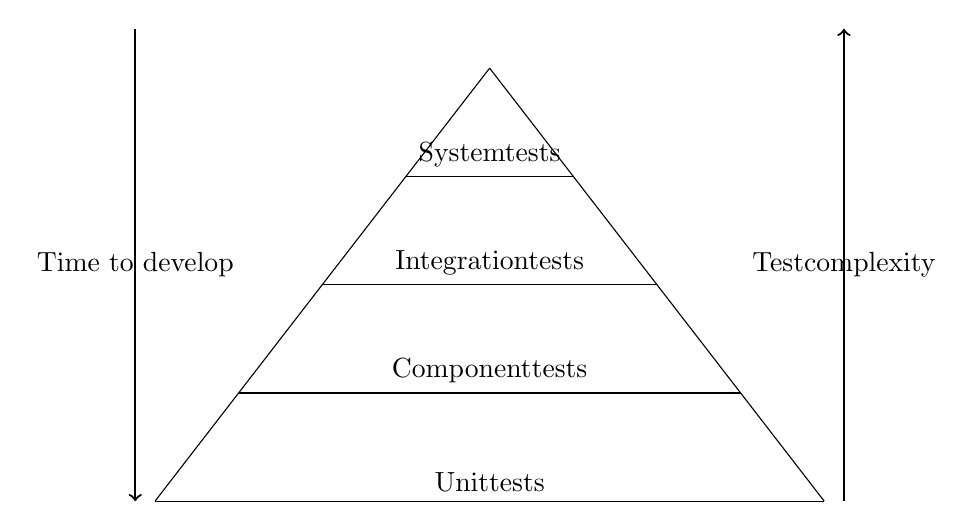
\begin{tikzpicture}
                \coordinate (A) at (-4.25,-1) {};
                \coordinate (B) at ( 4.25,-1) {};
                \coordinate (C) at (0,4.5) {};
                \draw[name path=AC] (A) -- (C);
                \draw[name path=BC] (B) -- (C);
                \draw[name path=AB] (A) -- (B);
    
                \foreach \y/\A in {0/Unittests,1/Componenttests, 2/Integrationtests, 3/Systemtests} {
                    \draw ($(A)!\y/4!(C)$) -- ($(B)!\y/4!(C)$) node[midway,above] {\A};\pause
                }
                \draw[thick, ->] (-4.5,5) -- (-4.5, -1) node[midway] {Time to develop};\pause
                \draw[thick, <-] (4.5,5) -- (4.5, -1) node[midway] {Testcomplexity};
            \end{tikzpicture}
        \end{frame}

        \subsectiontitle{Approaches}
        %short
        \begin{frame}{Continous Integration / Continous Delivery}
            \centering
            \begin{figure}
                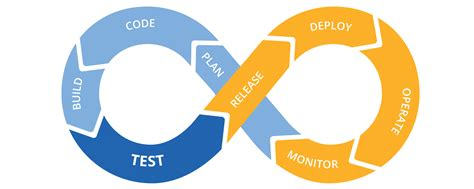
\includegraphics[width=12cm]{./images/cicd.jpeg}
            \end{figure}
        \end{frame}
        %short
        \begin{frame}{Test driven development}
            \centering
            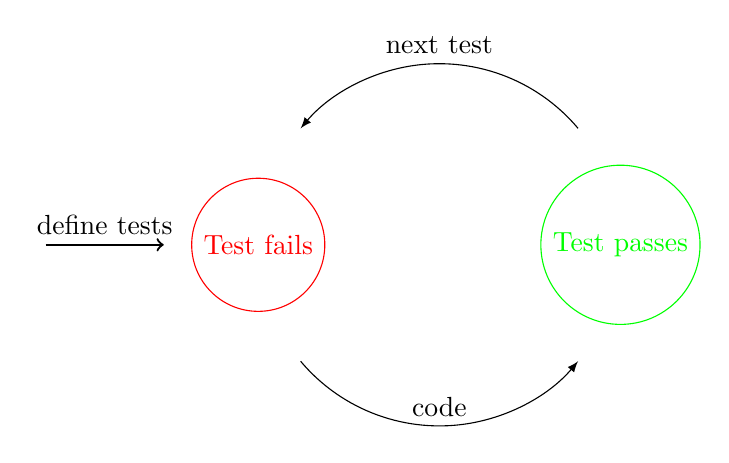
\begin{tikzpicture}
                \def \n {2}
                \def \radius {2.3cm}
                \def \margin {40}
                \draw[->,thick] (-5,0) -- (-3.5,0) node[midway, above] {define tests};
                \foreach \s/\A/\C/\N in {1/Test passes/green/next test,2/Test fails/red/code}
                {
                    \node[draw, circle,\C] at ({360/\n * (\s - 1)}:\radius) {\A};
                    \draw[->, >=latex] ({360/\n * (\s - 1)+\margin}:\radius) arc ({360/\n * (\s - 1)+\margin}:{360/\n * (\s)-\margin}:\radius) node[midway, above] {\N};
                }
            \end{tikzpicture}
        \end{frame}


    \sectiontitle{Boost.Test}

        \subsection{Basic usage}
        \begin{frame}{Structure}
            \lstinputlisting[language=c++]{scripts/structure.cpp}
        \end{frame}

        \begin{frame}{Assertion Levels}
            \begin{tabular}{c|c|c}
                assertion level &   error counter   &   test continuation   \\
                \hline
                warn    &       &   yes  \\
                check   &   ++  &   yes \\
                require &   ++  &   no  \\
            \end{tabular}
        \end{frame}

        % \begin{frame}{Basic Checks}
        %     \begin{itemize}
        %         \item  \inlinecpp{BOOST_<level>(predicate)}
        %         \item  \inlinecpp{BOOST_<level>_<GE,LE,GT,LT,NE>(left, right)}
        %         \item  \inlinecpp{BOOST_<level>_EQUAL(left, right)}
        %         \item  \inlinecpp{BOOST_IS_DEFINED(SYMBOL)}
        %     \end{itemize}
        % \end{frame}
        % \begin{frame}{Warn}
        %     \lstinputlisting[language=c++]{scripts/basic_warn.cpp}
        % \end{frame}
        % \begin{frame}{Check}
        %     \lstinputlisting[language=c++]{scripts/basic_checks.cpp}
        % \end{frame}
        % \begin{frame}{Require}
        %     \lstinputlisting[language=c++]{scripts/basic_require.cpp}
        % \end{frame}

        \begin{frame}{Float point comparison}
            \lstinputlisting[language=c++]{scripts/floatpoint_comparison.cpp}
        \end{frame}

        \begin{frame}{Exception handling}
            \lstinputlisting[language=c++]{scripts/exception_handling.cpp}      
        \end{frame}

        \subsection{Fixtures}
        \begin{frame}[plain]{Fixtures}
            \lstinputlisting[language=C++]{scripts/fixtures.cpp}
        \end{frame}

        \subsection{Templates}
        \begin{frame}[plain]{Templates}
            \lstinputlisting[language=C++]{scripts/templates.cpp}
        \end{frame}

    \sectiontitle{Testing}
        \subsection{Test executable}
        \begin{frame}{Test execution}
            \begin{itemize}
                \item add buildflags "--fprofile-arcs --ftest-coverage --fPIC" as well as no optimization for code coverage analysis
                \item build ug with UGTest and your plugin activated
                \item your plugin contains tests in a top level folder named "tests"
                \item executable named "ugtest\_unit" and "ugtest\_system" lands in ug4/bin
                \item \href{https://www.boost.org/doc/libs/1_58_0/libs/test/doc/html/utf/user-guide/runtime-config/reference.html}{list of params}
                \item example: \lstinline[language=bash]{ug4/bin $ ./ugtest_unit --log-level=ALL --log-format=HRF}
                \item Show result
            \end{itemize}
        \end{frame}
        
        \subsection{Jenkins}
        \begin{frame}{Automatization with Jenkins}
            \begin{itemize}
                \item Cobertura
                \item two builds one serial, one parallel -> two test runs
                \item Code coverage: gcovr can produce xml for cobertura
                \item needs log\_format=XML
            \end{itemize}
        \end{frame}

        \subsection{Docker}
        \begin{frame}{Automatization with Docker}
            \begin{itemize}
                \item Container stuff
                \item \href{https://github.com/Tobias-Trautmann/docker4ug4}{Dockerfile}
            \end{itemize}
        \end{frame}

    \sectiontitle{Additional}
    \begin{frame}{Open issues (?)}
        \begin{itemize}
            \item git branching \& releases
            \item naming conventions for tests
            \item definiton of done
            \item tooling
            \item error handling 
            \item design for testability
            \item test data
            \item mocking
        \end{itemize}
    \end{frame}
    \begin{frame}{Additional resources}
            \begin{itemize}
                \item \href{https://www.boost.org/doc/libs/1_58_0/libs/test/}{Boost.Test 1.58 documentation}
                \item \href{https://github.com/UG4/plugin_UGTest}{ugtests github}
                \item Antipatterns
                \item \href{https://docs.docker.com/}{Docker Documentation}
                \item \href{https://www.boost.org/doc/libs/1_73_0/libs/test/}{newest Boost.Test} %(often better documentation of already existing features)
                \item \href{https://www.dreckstool.de}{dreckstools}
            \end{itemize}
    \end{frame}

    \section{Refereneces}
    \begin{frame}{References}
        \begin{itemize}
            \item \href{https://en.wikipedia.org/wiki/Software_testing}{wiki}
            %definitly wrong pls fix
            \item Basiswissen Softwaretest
        \end{itemize}
    \end{frame}
\end{document}